\documentclass[a4paper, 12pt]{article}%тип документа

%отступы
\usepackage[left=2cm,right=2cm,top=2cm,bottom=3cm,bindingoffset=0cm]{geometry}

%Русский язык
\usepackage[T2A]{fontenc} %кодировка
\usepackage[utf8]{inputenc} %кодировка исходного кода
\usepackage[english,russian]{babel} %локализация и переносы

%Вставка картинок
\usepackage{wrapfig}
\usepackage{graphicx}
\graphicspath{{pictures/}}
\DeclareGraphicsExtensions{.pdf,.png,.jpg}

%оглавление
\usepackage{titlesec}
\titlespacing{\chapter}{0pt}{-30pt}{12pt}
\titlespacing{\section}{\parindent}{5mm}{5mm}
\titlespacing{\subsection}{\parindent}{5mm}{5mm}
\usepackage{setspace}

%Графики
\usepackage{multirow}
\usepackage{pgfplots}
\pgfplotsset{compat=1.9}

%Математика
\usepackage{amsmath, amsfonts, amssymb, amsthm, mathtools}

%Стиль страницы
\usepackage{fancyhdr}
\pagestyle{fancy}

\begin{document}

\begin{titlepage}

\begin{center}
%\vspace*{1cm}
\large\textbf{Московский Физико-Технический Институт}\\
\large\textbf{(государственный университет)}
\vfill
\line(1,0){430}\\[1mm]
\huge\textbf{Работа 4.3.2.}\\
\line(1,0){430}\\[1mm]
\vfill
\large Сибгатуллин Булат, ФРКТ\\
\end{center}

\end{titlepage}
\fancyhead[L] {Работа 4.3.2.}
\noindent \textbf{Цель работы:} \\
\indent изучение дифракции света на синусоидальной акустической решетке и наблюдение фазовой решетки методом темного поля.\\
\noindent \textbf{В работе используются:} \\
\indent оптическая скамья, осветитель, два длиннофокусных объектива, кювета с жидкостью, кварцевый излучатель с микрометрическим винтом, генератор звуковой частоты, линза, вертикальная нить на рейтере, микроскоп.

\section*{Описание работы}

\section*{Теоретическое введение}
	
	В работе используются оптическая скамья, осветитель, два длиннофокусных объектива, кювета с жидкостью, кварцевый излучатель с микрометрическим винтом, генератор звуковой частоты, линза, горизонтальная нить на рейтере, микроскоп. 
	
	При прохождении ультразвуковой волны через жидкость в ней возникают периодические неоднородности коэффициента преломления, создается фазовая решетка, которую мы считаем неподвижной ввиду малости скорости звука относительно скорости света. Показатель
	преломления n изменяется по закону:
	
	\begin{equation}\label{}
	n = n_0 (1 + m \cos \Omega x)
	\end{equation}
	
	Здесь $ \Omega = 2 \pi / \Lambda $ --- волновое число для ультразвуковой волны, $ m $ --- глубина модуляции $ n $ $ (m \ll 1 $).
	
	Положим фазу $ \phi $ колебаний световой волны на передней стенке кюветы равной нулю, тогда на задней поверхности она равна:
	
	\begin{equation}\label{}
	\phi  = k n L = \phi_0 (1 + m \cos \Omega x)
	\end{equation}
	
	Здесь $ L $ --- толщина жидкости в кювете, $ k = 2 \pi / \lambda $ --- волновое число для света.
	
	После прохождения через кювету световое поле есть совокупность плоских волн, распространяющихся под углами $ \theta $, соответствующими максимумам в дифракции Фраунгофера:
	
\begin{equation}\label{}	
	\Lambda \sin \theta_m = m \lambda
\end{equation}

	Этот эффект проиллюстрирован на рисунке 1.
	\begin{figure}[h!]
		\centering	
		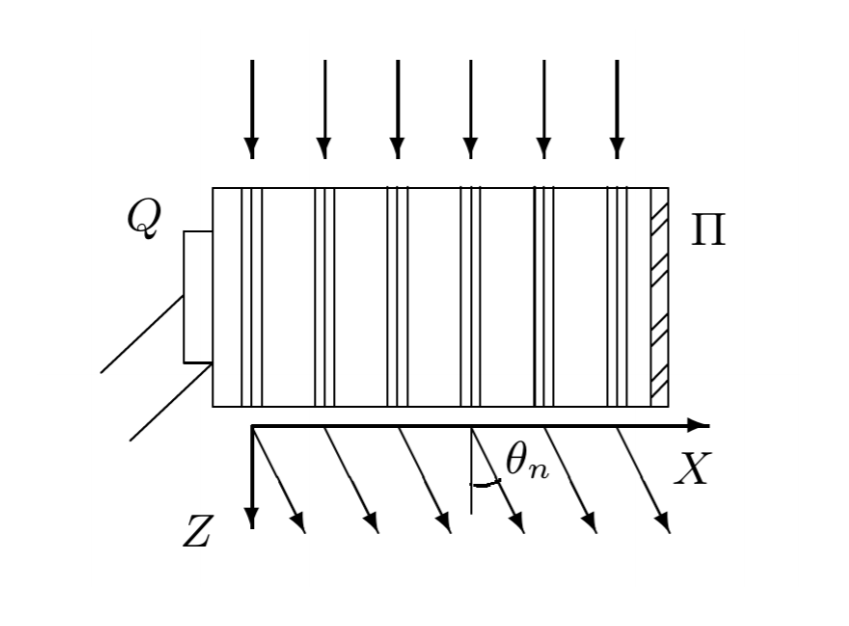
\includegraphics[width=0.3\textwidth]{images/wave.png}
		\caption{Дифракция световых волн на акустической решетке}
		\label{diff}
	\end{figure}
    Зная положение дифракционных максимумов, по формуле (1) легко определить длину ультразвуковой волны, учитывая малость $ \theta $: $ \sin \theta \approx \theta \approx l_m /F  $, где $ l_m $ --- расстояние от нулевого до последнего видимого максимума, $ F $ --- фокусное расстояние линзы. Тогда получим:
    	
    	\begin{equation}\label{}
    	 \Lambda = m \lambda F/ l_m 
    	\end{equation}
    	Скорость ультразвуковых волн в жидкости, где $ \nu $ --- частота колебаний излучателя:
    	
    \begin{equation}\label{}
    	v = \Lambda \nu 
    \end{equation}
    
    \textbf{Схема установки. }Схема установки приведена на рисунке 2. Источник света Л через светофильтр Ф и конденсор К освещает вертикальную щель $ S $, находящуюся в фокусе объектива $ O_1 $. После объектива параллельный световой пучок проходит через кювету С перпендикулярно акустической решетке, и дифракционная картина собирается в фокальной плоскости объектива $ O_2 $ , наблюдается при помощи микроскопа М.

    Предварительную настройку установки произведем в соответствии с инструкцией с зеленым фильтром, далее в работе используется красный.
    
    	\begin{figure}[h!]
    	\centering	
    	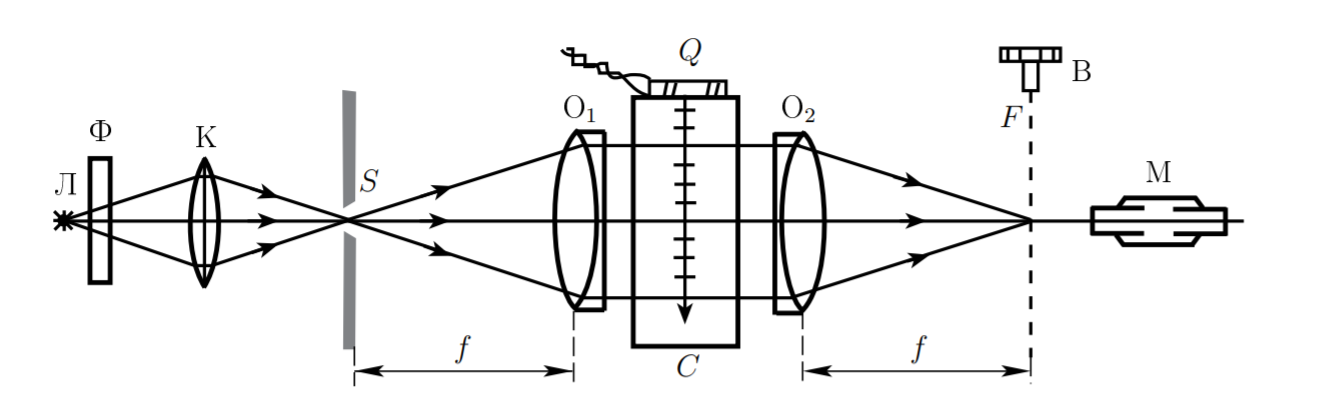
\includegraphics[width=0.7\textwidth]{images/stand.png}
    	\caption{Схема для наблюдения дифракции на акустической решетке}
    	\label{shema1}
    \end{figure}
    
    Параметры установки: фокусное расстояние объектива $F = 30 $ см, одно деление винта микроскопа составляет 20~мкм, полоса пропускания фильтра \mbox{$\lambda = 6400\pm 200$ Å}.
    

\section*{Ход работы}

\subsection*{Определение скорости ультразвука по дифракционной картине}

\begin{enumerate}

\item Соберем схему согласно рис.2 и настроим ее так, чтобы в объективе была видна дифракционная картина:

\begin{figure}[h!]
    \centering	
    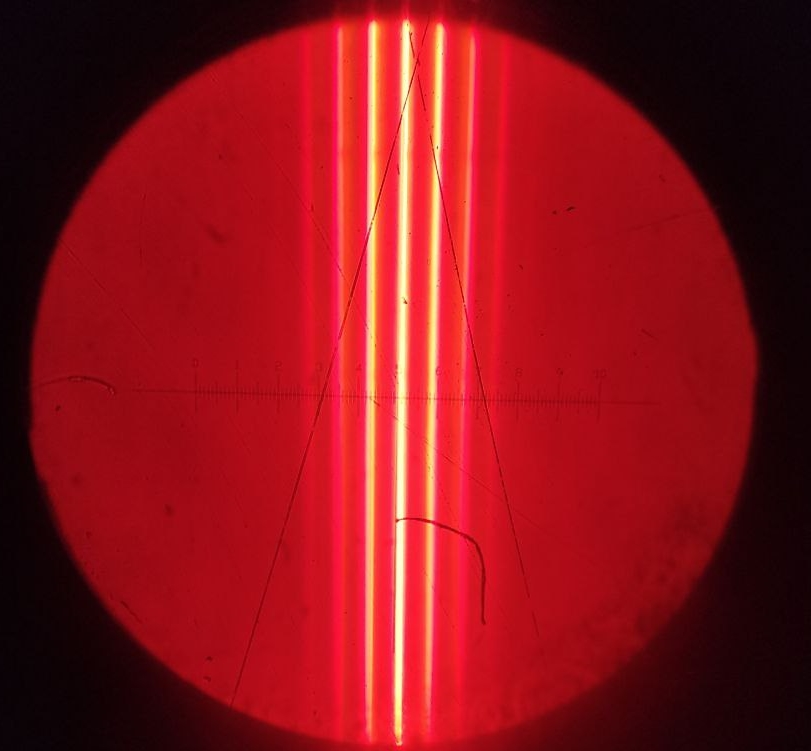
\includegraphics[width=0.7\textwidth]{images/1_1.jpg}
    \caption{Изображение дифракционных полос в объективе}
    \label{1_1}
\end{figure}

\item Измерим положения $x_m$ шести-восьми дифракционных максимумов с помощью поперечного микрометрического винта микроскопа, повторим измерения для 3-4-х частот в диапазоне от одного до 6-ти МГц.

\[f = 1,152 \: \text{МГц}\]

\begin{center}
\begin{tabular}{|c|c|c|c|c|c|c|c|}
\hline 
m & 3 & 2 & 1 & 0 & -1 & -2 & -3 \\ 
\hline 
$x,$ мкм & 1184 & 1036 & 888 & 744 & 600 & 424 & 268 \\ 
\hline 
\end{tabular} 
\end{center}

\[f = 3,946 \: \text{МГц}\]

\begin{center}
\begin{tabular}{|c|c|c|c|c|c|}
\hline 
m & -2 & -1 & 0 & 1 & 2 \\ 
\hline 
$x,$ мкм & 112 & 592 & 1120 & 1628 & 2140 \\ 
\hline 
\end{tabular} 
\end{center}

\[f = 1,812 \: \text{МГц}\]

\begin{center}
\begin{tabular}{|c|c|c|c|c|c|}
\hline 
m & -2 & -1 & 0 & 1 & 2 \\ 
\hline 
$x,$ мкм & 240 & 480 & 696 & 992 & 1176 \\ 
\hline 
\end{tabular} 
\end{center}

\[f = 4,6 \: \text{МГц}\]

\begin{center}
\begin{tabular}{|c|c|c|c|}
\hline 
m & -1 & 0 & 1 \\ 
\hline 
$x,$ мкм & 148 & 696 & 1316 \\ 
\hline 
\end{tabular} 
\end{center}

\[f = 6,16 \: \text{МГц}\]

\begin{center}
\begin{tabular}{|c|c|c|c|}
\hline 
m & -1 & 0 & 1 \\ 
\hline 
$x,$ мкм & 364 & 1184 & 2012 \\ 
\hline 
\end{tabular} 
\end{center}

\item Построим графики зависимости $x_m / m = \bigtriangleup x_m / \bigtriangleup m$ для каждой частоты. Получим линейные зависимость вида $y = ax + b$, в нашем случае $x_m / m = a$:

\[f = 1,152 \: \text{МГц} \Rightarrow a = 152,1 \pm 2,1 \: \text{мкм}\]

\[f = 3,946 \: \text{МГц} \Rightarrow a = 509,2 \pm 3,9\: \text{мкм}\]

\[f = 1,812 \: \text{МГц} \Rightarrow a = 238,4 \pm 8,4\: \text{мкм}\]

\[f = 4,6 \: \text{МГц} \Rightarrow a = 584 \pm 20\: \text{мкм}\]

\[f = 6,16 \: \text{МГц} \Rightarrow a = 842 \pm 2,3\: \text{мкм}\]

\begin{figure}[h!]
    \centering	
    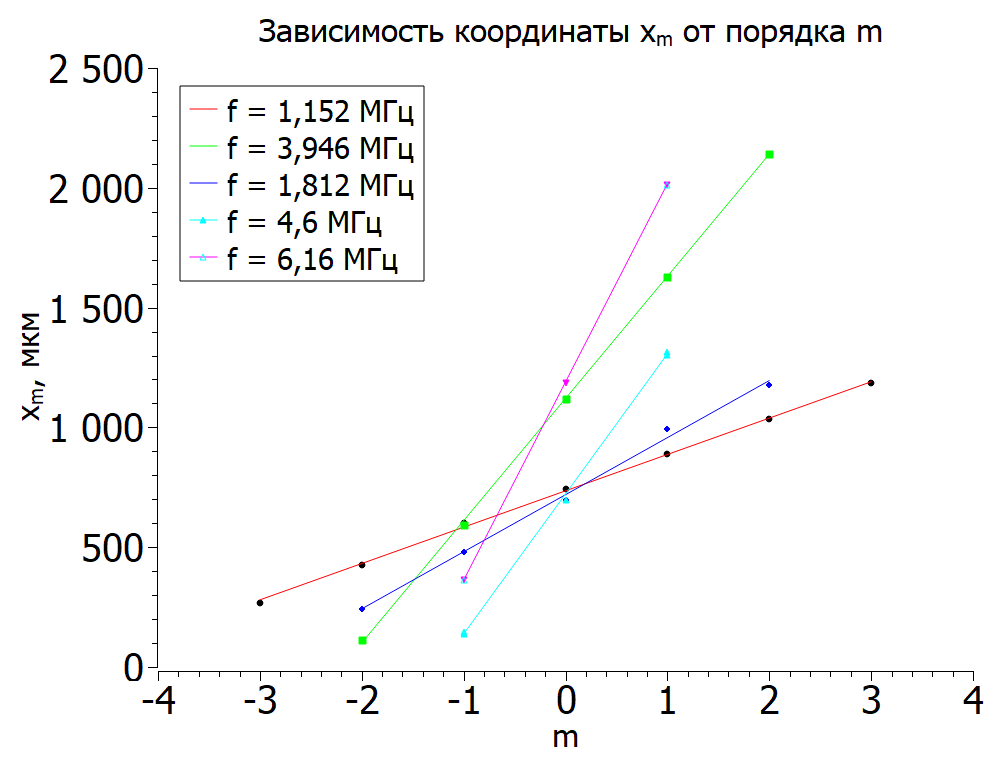
\includegraphics[width=0.7\textwidth]{images/graph_1.png}
    \caption{Графики зависимости $x_m / m$}
    \label{graph_1}
\end{figure}

\item Найдем длину $\Lambda$ УЗ-волны по формуле:

\[\Lambda = \frac{m}{l_m}F\lambda = \frac{F \lambda}{a},\]

где $a = a(f)$, а $\lambda = 640 \pm 20$ мкм и $F = 0,3$ м. Построим таблицу и график по получившимся данным:

\begin{center}
\begin{tabular}{|c|c|c|c|c|c|}
\hline 
$\Lambda,$ мкм & 228 & 329 & 377 & 807 & 1263 \\ 
\hline
$\sigma_{\Lambda},$ мкм & 2 & 11 & 3 & 28 & 17 \\ 
\hline 
$1/ \nu ,$ мкс & 0,1623 & 0,2174 & 0.2534 & 0,5519 & 0,8681 \\ 
\hline 
\end{tabular} 
\end{center}

\begin{figure}[h!]
    \centering	
    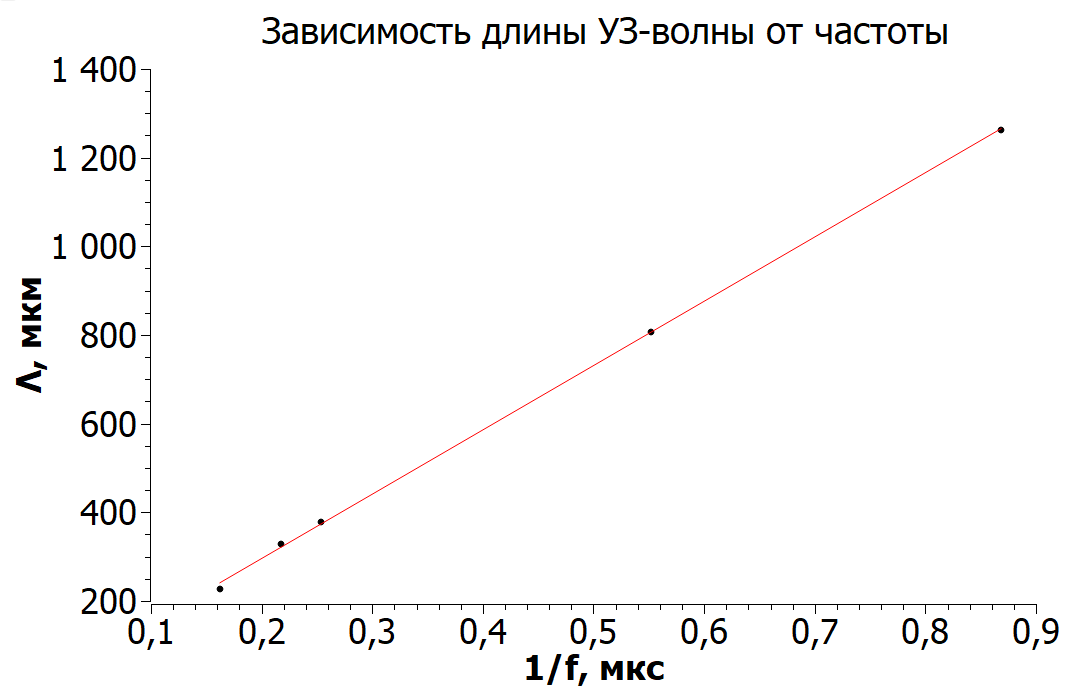
\includegraphics[width=0.7\textwidth]{images/graph_2.png}
    \caption{Зависимость длины УЗ-волны от частоты}
    \label{graph_2}
\end{figure}

В итоге получим зависимость вида $y = ax+b$, где $a = 1452 \pm 53$. Зная, что:

\[v = \Lambda * \nu = \frac{\Lambda}{1/\nu},\]

получаем, что $a= v$, где $v$ - скорость ультразвуковых волн в жилкости и она равна:

\[v = 1452 \pm 53 \: \text{м/с}\]

Для сравнения, табличное значение составляет $v = 1490$ м/с.

\subsection*{Определение скорость ультразвука методом темного поля}

\item Для перехода к методу темного поля отодвинем микроскоп от щели и разметим в промежутке между ними дополнительную линзу. Поднимем излучатель над кюветой, опустим в воду квадратную сетку и прижмем ее к задней по ходу луча стенке кюветы. Центрируя линзу найдем изображение сетки в микроскопе:

\begin{figure}[h!]
    \centering	
    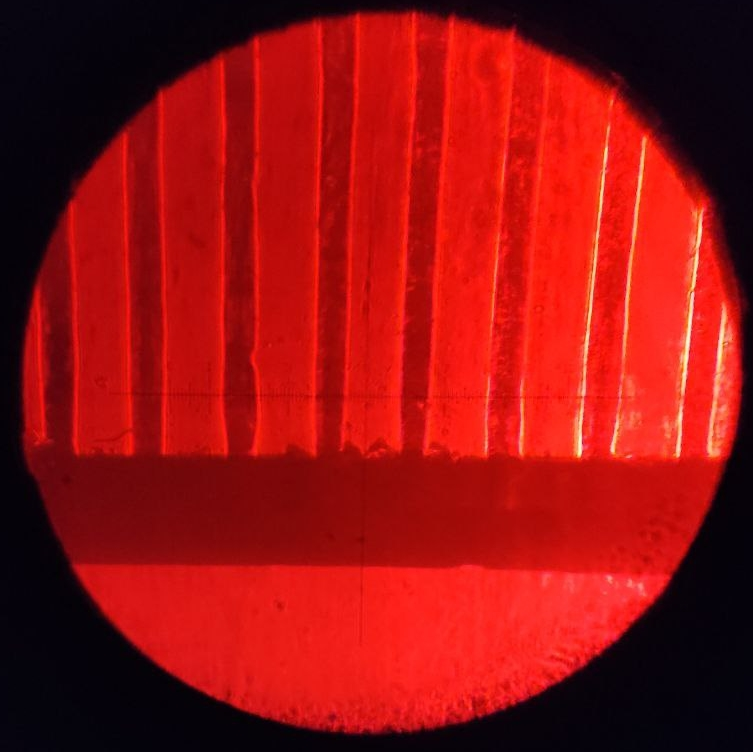
\includegraphics[width=0.7\textwidth]{images/2_1.jpg}
    \caption{Изображение сетки}
    \label{2_1}
\end{figure}

\newpage
Зафиксируем координаты совпадающих штрихов окулярной шкалы и сетки - 7 штрихов сетки соответствуют 9,1 делениям на окулярной шкале.

\item Для наблюдения акустической решетки установим рабочую нирину щели (20-30 мкм) и закроем нулевой дифракционный максимум проволочкой. Уберем калибровочную сетку и варьируя частоту увидим акустическую решетку в микроскоп:

\begin{figure}[h!]
    \centering	
    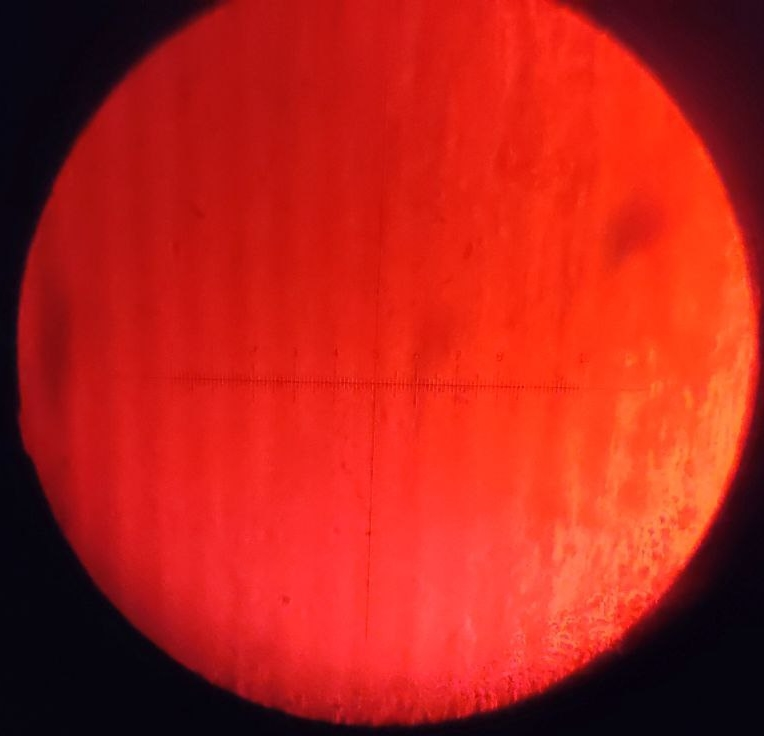
\includegraphics[width=0.7\textwidth]{images/3_1.jpg}
    \caption{Изображение звуковой решетки}
    \label{3_1}
\end{figure}

\end{enumerate}

\newpage
\section*{Вывод}

Изучили явление дифракции света на ультразвуковой волне в воде. Сняли зависимость длины волны ультразвука от его частоты, и по этим параметрам получили значение скорости ультразвука в воде. Полученное значение совпало с табличным. Также пронаблюдали акустическую решетку.

\end{document}